\documentclass[]{article}
\usepackage{lmodern}
\usepackage{amssymb,amsmath}
\usepackage{ifxetex,ifluatex}
\usepackage{fixltx2e} % provides \textsubscript
\ifnum 0\ifxetex 1\fi\ifluatex 1\fi=0 % if pdftex
  \usepackage[T1]{fontenc}
  \usepackage[utf8]{inputenc}
\else % if luatex or xelatex
  \ifxetex
    \usepackage{mathspec}
  \else
    \usepackage{fontspec}
  \fi
  \defaultfontfeatures{Ligatures=TeX,Scale=MatchLowercase}
\fi
% use upquote if available, for straight quotes in verbatim environments
\IfFileExists{upquote.sty}{\usepackage{upquote}}{}
% use microtype if available
\IfFileExists{microtype.sty}{%
\usepackage{microtype}
\UseMicrotypeSet[protrusion]{basicmath} % disable protrusion for tt fonts
}{}
\usepackage[margin=1in]{geometry}
\usepackage{hyperref}
\hypersetup{unicode=true,
            pdftitle={Processing, cleaning and saving NZ GREEN Grid project 1 minute electricity consumption data},
            pdfauthor={Ben Anderson (b.anderson@soton.ac.uk, @dataknut)},
            pdfborder={0 0 0},
            breaklinks=true}
\urlstyle{same}  % don't use monospace font for urls
\usepackage{color}
\usepackage{fancyvrb}
\newcommand{\VerbBar}{|}
\newcommand{\VERB}{\Verb[commandchars=\\\{\}]}
\DefineVerbatimEnvironment{Highlighting}{Verbatim}{commandchars=\\\{\}}
% Add ',fontsize=\small' for more characters per line
\usepackage{framed}
\definecolor{shadecolor}{RGB}{248,248,248}
\newenvironment{Shaded}{\begin{snugshade}}{\end{snugshade}}
\newcommand{\KeywordTok}[1]{\textcolor[rgb]{0.13,0.29,0.53}{\textbf{#1}}}
\newcommand{\DataTypeTok}[1]{\textcolor[rgb]{0.13,0.29,0.53}{#1}}
\newcommand{\DecValTok}[1]{\textcolor[rgb]{0.00,0.00,0.81}{#1}}
\newcommand{\BaseNTok}[1]{\textcolor[rgb]{0.00,0.00,0.81}{#1}}
\newcommand{\FloatTok}[1]{\textcolor[rgb]{0.00,0.00,0.81}{#1}}
\newcommand{\ConstantTok}[1]{\textcolor[rgb]{0.00,0.00,0.00}{#1}}
\newcommand{\CharTok}[1]{\textcolor[rgb]{0.31,0.60,0.02}{#1}}
\newcommand{\SpecialCharTok}[1]{\textcolor[rgb]{0.00,0.00,0.00}{#1}}
\newcommand{\StringTok}[1]{\textcolor[rgb]{0.31,0.60,0.02}{#1}}
\newcommand{\VerbatimStringTok}[1]{\textcolor[rgb]{0.31,0.60,0.02}{#1}}
\newcommand{\SpecialStringTok}[1]{\textcolor[rgb]{0.31,0.60,0.02}{#1}}
\newcommand{\ImportTok}[1]{#1}
\newcommand{\CommentTok}[1]{\textcolor[rgb]{0.56,0.35,0.01}{\textit{#1}}}
\newcommand{\DocumentationTok}[1]{\textcolor[rgb]{0.56,0.35,0.01}{\textbf{\textit{#1}}}}
\newcommand{\AnnotationTok}[1]{\textcolor[rgb]{0.56,0.35,0.01}{\textbf{\textit{#1}}}}
\newcommand{\CommentVarTok}[1]{\textcolor[rgb]{0.56,0.35,0.01}{\textbf{\textit{#1}}}}
\newcommand{\OtherTok}[1]{\textcolor[rgb]{0.56,0.35,0.01}{#1}}
\newcommand{\FunctionTok}[1]{\textcolor[rgb]{0.00,0.00,0.00}{#1}}
\newcommand{\VariableTok}[1]{\textcolor[rgb]{0.00,0.00,0.00}{#1}}
\newcommand{\ControlFlowTok}[1]{\textcolor[rgb]{0.13,0.29,0.53}{\textbf{#1}}}
\newcommand{\OperatorTok}[1]{\textcolor[rgb]{0.81,0.36,0.00}{\textbf{#1}}}
\newcommand{\BuiltInTok}[1]{#1}
\newcommand{\ExtensionTok}[1]{#1}
\newcommand{\PreprocessorTok}[1]{\textcolor[rgb]{0.56,0.35,0.01}{\textit{#1}}}
\newcommand{\AttributeTok}[1]{\textcolor[rgb]{0.77,0.63,0.00}{#1}}
\newcommand{\RegionMarkerTok}[1]{#1}
\newcommand{\InformationTok}[1]{\textcolor[rgb]{0.56,0.35,0.01}{\textbf{\textit{#1}}}}
\newcommand{\WarningTok}[1]{\textcolor[rgb]{0.56,0.35,0.01}{\textbf{\textit{#1}}}}
\newcommand{\AlertTok}[1]{\textcolor[rgb]{0.94,0.16,0.16}{#1}}
\newcommand{\ErrorTok}[1]{\textcolor[rgb]{0.64,0.00,0.00}{\textbf{#1}}}
\newcommand{\NormalTok}[1]{#1}
\usepackage{longtable,booktabs}
\usepackage{graphicx,grffile}
\makeatletter
\def\maxwidth{\ifdim\Gin@nat@width>\linewidth\linewidth\else\Gin@nat@width\fi}
\def\maxheight{\ifdim\Gin@nat@height>\textheight\textheight\else\Gin@nat@height\fi}
\makeatother
% Scale images if necessary, so that they will not overflow the page
% margins by default, and it is still possible to overwrite the defaults
% using explicit options in \includegraphics[width, height, ...]{}
\setkeys{Gin}{width=\maxwidth,height=\maxheight,keepaspectratio}
\IfFileExists{parskip.sty}{%
\usepackage{parskip}
}{% else
\setlength{\parindent}{0pt}
\setlength{\parskip}{6pt plus 2pt minus 1pt}
}
\setlength{\emergencystretch}{3em}  % prevent overfull lines
\providecommand{\tightlist}{%
  \setlength{\itemsep}{0pt}\setlength{\parskip}{0pt}}
\setcounter{secnumdepth}{0}
% Redefines (sub)paragraphs to behave more like sections
\ifx\paragraph\undefined\else
\let\oldparagraph\paragraph
\renewcommand{\paragraph}[1]{\oldparagraph{#1}\mbox{}}
\fi
\ifx\subparagraph\undefined\else
\let\oldsubparagraph\subparagraph
\renewcommand{\subparagraph}[1]{\oldsubparagraph{#1}\mbox{}}
\fi

%%% Use protect on footnotes to avoid problems with footnotes in titles
\let\rmarkdownfootnote\footnote%
\def\footnote{\protect\rmarkdownfootnote}

%%% Change title format to be more compact
\usepackage{titling}

% Create subtitle command for use in maketitle
\newcommand{\subtitle}[1]{
  \posttitle{
    \begin{center}\large#1\end{center}
    }
}

\setlength{\droptitle}{-2em}
  \title{Processing, cleaning and saving NZ GREEN Grid project 1 minute
electricity consumption data}
  \pretitle{\vspace{\droptitle}\centering\huge}
  \posttitle{\par}
  \author{Ben Anderson
(\href{mailto:b.anderson@soton.ac.uk}{\nolinkurl{b.anderson@soton.ac.uk}},
\texttt{@dataknut})}
  \preauthor{\centering\large\emph}
  \postauthor{\par}
  \predate{\centering\large\emph}
  \postdate{\par}
  \date{Last run at: 2018-05-01 17:32:39}


\begin{document}
\maketitle

{
\setcounter{tocdepth}{2}
\tableofcontents
}
\newpage

\section{Citation}\label{citation}

If you wish to use any of the material from this report please cite as:

\begin{itemize}
\tightlist
\item
  Anderson, B. (2018) Processing, cleaning and saving NZ GREEN Grid
  project 1 minute electricity consumption data, University of Otago:
  Dunedin, NZ.
\end{itemize}

\newpage

\section{Introduction}\label{introduction}

Report circulation:

\begin{itemize}
\tightlist
\item
  Restricted to:
  \href{https://www.otago.ac.nz/centre-sustainability/research/energy/otago050285.html}{NZ
  GREEn Grid} project partners and contractors.
\end{itemize}

\subsection{Purpose}\label{purpose}

This report is intended to:

\begin{itemize}
\tightlist
\item
  load and clean the project electricity consumption data (Grid Spy)
\item
  save the cleaned data out as a single file per household
\item
  produce summary data quality statistics
\end{itemize}

\subsection{Requirements:}\label{requirements}

\begin{itemize}
\tightlist
\item
  grid spy 1 minute data downloads
\end{itemize}

\subsection{History}\label{history}

Generally tracked via our git.soton
\href{https://git.soton.ac.uk/ba1e12/nzGREENGrid}{repo}.

\subsection{Support}\label{support}

This work was supported by:

\begin{itemize}
\tightlist
\item
  The \href{https://www.otago.ac.nz/}{University of Otago}
\item
  The New Zealand \href{http://www.mbie.govt.nz/}{Ministry of Business,
  Innovation and Employment (MBIE)}
\item
  \href{http://www.energy.soton.ac.uk/tag/spatialec/}{SPATIALEC} - a
  \href{http://ec.europa.eu/research/mariecurieactions/about-msca/actions/if/index_en.htm}{Marie
  Skłodowska-Curie Global Fellowship} based at the University of Otago's
  \href{http://www.otago.ac.nz/centre-sustainability/staff/otago673896.html}{Centre
  for Sustainability} (2017-2019) \& the University of Southampton's
  Sustainable Energy Research Group (2019-202).
\end{itemize}

This work uis (c) 2018 the University of Southampton.

\section{Obtain listing of files}\label{obtain-listing-of-files}

In this section we generate a listing of all 1 minute data files that we
have received. If we are running over the complete dataset then we will
be using data from:

\begin{itemize}
\tightlist
\item
  /hum-csafe/Research Projects/GREEN Grid/\_RAW DATA/GridSpyData/
\end{itemize}

In this run we are using data from:

\begin{itemize}
\tightlist
\item
  \textasciitilde{}/Data/NZGreenGrid/gridspy/1min\_orig/
\end{itemize}

If these do not match then this may be a test run.

\begin{Shaded}
\begin{Highlighting}[]
\KeywordTok{print}\NormalTok{(}\KeywordTok{paste0}\NormalTok{(}\StringTok{"Looking for 1 minute data using pattern = "}\NormalTok{, pattern1Min, }\StringTok{" in "}\NormalTok{, fpath))}
\end{Highlighting}
\end{Shaded}

\begin{verbatim}
## [1] "Looking for 1 minute data using pattern = *at1.csv$ in ~/Data/NZGreenGrid/gridspy/1min_orig/"
\end{verbatim}

\begin{Shaded}
\begin{Highlighting}[]
\NormalTok{fListCompleteDT <-}\StringTok{ }\KeywordTok{as.data.table}\NormalTok{(}\KeywordTok{list.files}\NormalTok{(}\DataTypeTok{path =}\NormalTok{ fpath, }\DataTypeTok{pattern =}\NormalTok{ pattern1Min, }\CommentTok{# use the default pattern to filter e.g. 1m from 30s files}
                                            \DataTypeTok{recursive =} \OtherTok{TRUE}\NormalTok{))}
\ControlFlowTok{if}\NormalTok{(}\KeywordTok{nrow}\NormalTok{(fListCompleteDT) }\OperatorTok{==}\StringTok{ }\DecValTok{0}\NormalTok{)\{}
  \KeywordTok{stop}\NormalTok{(}\KeywordTok{paste0}\NormalTok{(}\StringTok{"No matching data files found, please check your path ("}\NormalTok{, fpath, }\StringTok{") or your search pattern ("}\NormalTok{, pattern1Min, }\StringTok{")"}\NormalTok{))}
\NormalTok{\} }\ControlFlowTok{else}\NormalTok{ \{}
  \KeywordTok{print}\NormalTok{(}\KeywordTok{paste0}\NormalTok{(}\StringTok{"Processing file list and getting file meta-data (please be patient)"}\NormalTok{))}
\NormalTok{  fListCompleteDT <-}\StringTok{ }\NormalTok{fListCompleteDT[, }\KeywordTok{c}\NormalTok{(}\StringTok{"hhID"}\NormalTok{,}\StringTok{"fileName"}\NormalTok{) }\OperatorTok{:}\ErrorTok{=}\StringTok{ }\KeywordTok{tstrsplit}\NormalTok{(V1, }\StringTok{"/"}\NormalTok{)]}
\NormalTok{  fListCompleteDT <-}\StringTok{ }\NormalTok{fListCompleteDT[, fullPath }\OperatorTok{:}\ErrorTok{=}\StringTok{ }\KeywordTok{paste0}\NormalTok{(fpath, hhID,}\StringTok{"/"}\NormalTok{,fileName)]}
  
  \ControlFlowTok{for}\NormalTok{(f }\ControlFlowTok{in}\NormalTok{ fListCompleteDT[,fullPath])\{}
\NormalTok{    rf <-}\StringTok{ }\KeywordTok{path.expand}\NormalTok{(f) }\CommentTok{# just in case of ~ etc}
\NormalTok{    fsize <-}\StringTok{ }\KeywordTok{file.size}\NormalTok{(rf)}
\NormalTok{    fmtime <-}\StringTok{ }\KeywordTok{ymd_hms}\NormalTok{(}\KeywordTok{file.mtime}\NormalTok{(rf), }\DataTypeTok{tz =} \StringTok{"Pacific/Auckland"}\NormalTok{) }\CommentTok{# requires lubridate}
\NormalTok{    fListCompleteDT <-}\StringTok{ }\NormalTok{fListCompleteDT[fullPath }\OperatorTok{==}\StringTok{ }\NormalTok{f, fSize }\OperatorTok{:}\ErrorTok{=}\StringTok{ }\NormalTok{fsize]}
\NormalTok{    fListCompleteDT <-}\StringTok{ }\NormalTok{fListCompleteDT[fullPath }\OperatorTok{==}\StringTok{ }\NormalTok{f, fMTime }\OperatorTok{:}\ErrorTok{=}\StringTok{ }\NormalTok{fmtime]}
\NormalTok{    fListCompleteDT <-}\StringTok{ }\NormalTok{fListCompleteDT[fullPath }\OperatorTok{==}\StringTok{ }\NormalTok{f, fMDate }\OperatorTok{:}\ErrorTok{=}\StringTok{ }\KeywordTok{as.Date}\NormalTok{(fmtime)]}
\NormalTok{  \}}
\NormalTok{  ofile <-}\StringTok{ }\KeywordTok{paste0}\NormalTok{(outPath, indexFile)}
  \KeywordTok{print}\NormalTok{(}\KeywordTok{paste0}\NormalTok{(}\StringTok{"Saving 1 minute data files metadata to "}\NormalTok{, ofile))}
  \KeywordTok{write.csv}\NormalTok{(fListCompleteDT, ofile)}
  \KeywordTok{print}\NormalTok{(}\StringTok{"Done"}\NormalTok{)}
\NormalTok{\}}
\end{Highlighting}
\end{Shaded}

\begin{verbatim}
## [1] "Processing file list and getting file meta-data (please be patient)"
## [1] "Saving 1 minute data files metadata to ~/Data/NZGreenGrid/gridspy/consolidated/fListCompleteDT.csv"
## [1] "Done"
\end{verbatim}

Overall we have 1913 files from 4 households. The following chart shows
the distribution of these files over time using their sizes. Note that
white indicates the presence of small files which may not contain
observations.

\begin{Shaded}
\begin{Highlighting}[]
\NormalTok{myCaption <-}\StringTok{ }\KeywordTok{paste0}\NormalTok{(}\StringTok{"Data source: "}\NormalTok{, fpath,}
                    \StringTok{"}\CharTok{\textbackslash{}n}\StringTok{Using data received up to "}\NormalTok{, }\KeywordTok{Sys.Date}\NormalTok{())}

\NormalTok{plotDT <-}\StringTok{ }\NormalTok{fListCompleteDT[, .(}\DataTypeTok{nFiles =}\NormalTok{ .N,}
                              \DataTypeTok{meanfSize =} \KeywordTok{mean}\NormalTok{(fSize)), }
\NormalTok{                          keyby =}\StringTok{ }\NormalTok{.(hhID, }\DataTypeTok{date =} \KeywordTok{as.Date}\NormalTok{(fMDate))]}

\CommentTok{#>> All files plots ----}
\KeywordTok{ggplot}\NormalTok{(plotDT, }\KeywordTok{aes}\NormalTok{( }\DataTypeTok{x =}\NormalTok{ date, }\DataTypeTok{y =}\NormalTok{ hhID, }\DataTypeTok{fill =} \KeywordTok{log}\NormalTok{(meanfSize))) }\OperatorTok{+}
\StringTok{  }\KeywordTok{geom_tile}\NormalTok{() }\OperatorTok{+}
\StringTok{  }\KeywordTok{scale_fill_gradient}\NormalTok{(}\DataTypeTok{low =} \StringTok{"white"}\NormalTok{, }\DataTypeTok{high =} \StringTok{"black"}\NormalTok{) }\OperatorTok{+}\StringTok{ }
\StringTok{  }\KeywordTok{scale_x_date}\NormalTok{(}\DataTypeTok{date_labels =} \StringTok{"%Y %b"}\NormalTok{, }\DataTypeTok{date_breaks =} \StringTok{"1 month"}\NormalTok{) }\OperatorTok{+}
\StringTok{  }\KeywordTok{theme}\NormalTok{(}\DataTypeTok{axis.text.x =} \KeywordTok{element_text}\NormalTok{(}\DataTypeTok{angle =} \DecValTok{90}\NormalTok{, }\DataTypeTok{vjust =} \FloatTok{0.5}\NormalTok{, }\DataTypeTok{hjust =} \FloatTok{0.5}\NormalTok{)) }\OperatorTok{+}\StringTok{ }
\StringTok{  }\KeywordTok{labs}\NormalTok{(}\DataTypeTok{title =} \StringTok{"Mean file size of all grid spy data files received per day"}\NormalTok{,}
       \DataTypeTok{caption =} \KeywordTok{paste0}\NormalTok{(myCaption, }
                        \StringTok{"}\CharTok{\textbackslash{}n}\StringTok{Log file size used as some files are full year data"}\NormalTok{)}
    
\NormalTok{  )}
\end{Highlighting}
\end{Shaded}

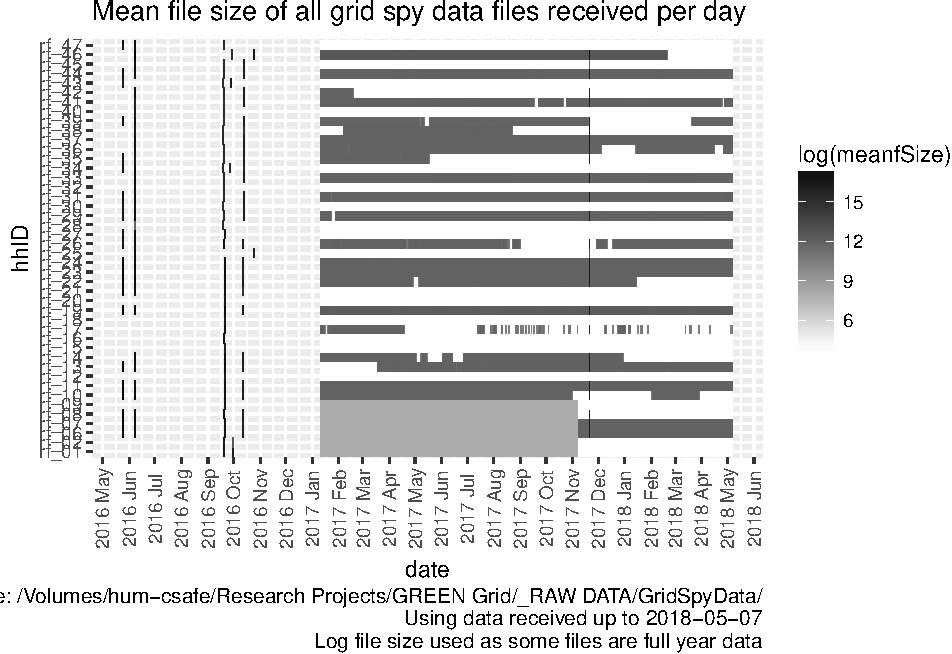
\includegraphics{processNZGGElecCons1minData_files/figure-latex/allFileSizesPlot-1.pdf}

\begin{Shaded}
\begin{Highlighting}[]
\KeywordTok{ggsave}\NormalTok{(}\KeywordTok{paste0}\NormalTok{(outPath, }\StringTok{"gridSpyAllFileListSizeTilePlot.png"}\NormalTok{))}
\end{Highlighting}
\end{Shaded}

\begin{verbatim}
## Saving 6.5 x 4.5 in image
\end{verbatim}

\section{Load data files}\label{load-data-files}

In this section we load the data files that have a file size
\textgreater{} 3000 bytes. Things to note:

\begin{itemize}
\tightlist
\item
  We assume that any files smaller than this value have no observations.
  This is based on:

  \begin{itemize}
  \tightlist
  \item
    Manual inspection of several small files
  \item
    The identical (small) file sizes involved
  \item
    \emph{But} we should probably test the first few lines to double
    check\ldots{}
  \end{itemize}
\item
  We have to deal with at least 2 different date formats and quite a lot
  of duplication some of which causes the differnt date formats. The
  code to fix these is included below but see also our
  \href{https://git.soton.ac.uk/ba1e12/nzGREENGrid/issues?scope=all\&utf8=\%E2\%9C\%93\&state=all}{repo
  issues list}.
\end{itemize}

\begin{Shaded}
\begin{Highlighting}[]
\CommentTok{# > Load, process & save the ones which probably have data ----}

\NormalTok{hhIDs <-}\StringTok{ }\KeywordTok{unique}\NormalTok{(fListCompleteDT}\OperatorTok{$}\NormalTok{hhID) }\CommentTok{# list of household ids}
\NormalTok{hhStatDT <-}\StringTok{ }\KeywordTok{data.table}\NormalTok{() }\CommentTok{# stats collector}
\ControlFlowTok{for}\NormalTok{(hh }\ControlFlowTok{in}\NormalTok{ hhIDs)\{}
  \KeywordTok{print}\NormalTok{(}\KeywordTok{paste0}\NormalTok{(}\StringTok{"Loading: "}\NormalTok{, hh))}
\NormalTok{  tempHhDT <-}\StringTok{ }\KeywordTok{data.table}\NormalTok{() }\CommentTok{# create data.table to hold file contents}
\NormalTok{  fListCompleteDT <-}\StringTok{ }\NormalTok{fListCompleteDT[, fileLoaded }\OperatorTok{:}\ErrorTok{=}\StringTok{ "No"}\NormalTok{]}
\NormalTok{  filesToLoad <-}\StringTok{ }\NormalTok{fListCompleteDT[hhID }\OperatorTok{==}\StringTok{ }\NormalTok{hh }\OperatorTok{&}\StringTok{ }\NormalTok{fSize }\OperatorTok{>}\StringTok{ }\NormalTok{dataThreshold, fullPath] }\CommentTok{# select the files that meet our size threshold}
  \ControlFlowTok{for}\NormalTok{(f }\ControlFlowTok{in}\NormalTok{ filesToLoad)\{}
    \CommentTok{#print(paste0("File size (", f, ") = ", fListCompleteDT[fullPath == f, fSize], " so probably OK")) # files under 3kb are probably empty}
    \CommentTok{# attempt to load the file}
\NormalTok{    tempDT <-}\StringTok{ }\KeywordTok{fread}\NormalTok{(f)}
    \CommentTok{#print("File loaded")}
    \CommentTok{# set some file stats}
\NormalTok{    fListCompleteDT <-}\StringTok{ }\NormalTok{fListCompleteDT[fullPath }\OperatorTok{==}\StringTok{ }\NormalTok{f, fileLoaded }\OperatorTok{:}\ErrorTok{=}\StringTok{ "Yes"}\NormalTok{]}
\NormalTok{    fListCompleteDT <-}\StringTok{ }\NormalTok{fListCompleteDT[fullPath }\OperatorTok{==}\StringTok{ }\NormalTok{f, nObs }\OperatorTok{:}\ErrorTok{=}\StringTok{ }\KeywordTok{nrow}\NormalTok{(tempDT)] }\CommentTok{# could include duplicates}
    \ControlFlowTok{if}\NormalTok{(}\KeywordTok{nrow}\NormalTok{(}\KeywordTok{select}\NormalTok{(tempDT, }\KeywordTok{contains}\NormalTok{(}\StringTok{"NZ"}\NormalTok{))) }\OperatorTok{>}\StringTok{ }\DecValTok{0}\NormalTok{)\{ }\CommentTok{# requires dplyr}
      \CommentTok{# => there is at least 1 column whose name contains NZ so we have NZ time}
      \CommentTok{#print("NZ time")}
      \KeywordTok{setnames}\NormalTok{(tempDT, }\StringTok{'date NZ'}\NormalTok{, }\StringTok{"date_NZ"}\NormalTok{)}
      \CommentTok{# Check the date format as it could be y-m-d or d/m/y :-(}
\NormalTok{      tempDT <-}\StringTok{ }\NormalTok{tempDT[, testDate }\OperatorTok{:}\ErrorTok{=}\StringTok{ }\KeywordTok{ifelse}\NormalTok{(}\KeywordTok{substr}\NormalTok{(date_NZ,}\DecValTok{2}\NormalTok{,}\DecValTok{2}\NormalTok{) }\OperatorTok{==}\StringTok{ "/"} \OperatorTok{|}\StringTok{ }\CommentTok{# day is 1 digit}
\StringTok{                                              }\KeywordTok{substr}\NormalTok{(date_NZ,}\DecValTok{3}\NormalTok{,}\DecValTok{3}\NormalTok{) }\OperatorTok{==}\StringTok{ "/"}\NormalTok{ , }\CommentTok{# day is 2 digits}
                                            \StringTok{"dmy"}\NormalTok{, }\StringTok{"ymd"}\NormalTok{)] }\CommentTok{# if there is a "/" then it is d/m/y}
      \CommentTok{# Now use that to correctly parse dates}
\NormalTok{      tempDT <-}\StringTok{ }\NormalTok{tempDT[testDate }\OperatorTok{==}\StringTok{ "ymd"}\NormalTok{, r_dateTime }\OperatorTok{:}\ErrorTok{=}\StringTok{ }\KeywordTok{ymd_hm}\NormalTok{(date_NZ, }\DataTypeTok{tz =} \StringTok{"Pacific/Auckland"}\NormalTok{)] }\CommentTok{# requires lubridate}
\NormalTok{      tempDT <-}\StringTok{ }\NormalTok{tempDT[testDate }\OperatorTok{==}\StringTok{ "dmy"}\NormalTok{, r_dateTime }\OperatorTok{:}\ErrorTok{=}\StringTok{ }\KeywordTok{dmy_hm}\NormalTok{(date_NZ, }\DataTypeTok{tz =} \StringTok{"Pacific/Auckland"}\NormalTok{)]}
\NormalTok{    \} }\ControlFlowTok{else}\NormalTok{ \{}
      \CommentTok{# we have UTC}
      \CommentTok{#print("UTC")}
      \KeywordTok{setnames}\NormalTok{(tempDT, }\StringTok{'date UTC'}\NormalTok{, }\StringTok{"date_UTC"}\NormalTok{)}
\NormalTok{      tempDT <-}\StringTok{ }\NormalTok{tempDT[, testDate }\OperatorTok{:}\ErrorTok{=}\StringTok{ }\KeywordTok{ifelse}\NormalTok{(}\KeywordTok{substr}\NormalTok{(date_UTC,}\DecValTok{2}\NormalTok{,}\DecValTok{2}\NormalTok{) }\OperatorTok{==}\StringTok{ "/"} \OperatorTok{|}\StringTok{ }\CommentTok{# day is 1 digit}
\StringTok{                                              }\KeywordTok{substr}\NormalTok{(date_UTC,}\DecValTok{3}\NormalTok{,}\DecValTok{3}\NormalTok{) }\OperatorTok{==}\StringTok{ "/"}\NormalTok{, }\CommentTok{# 2 digits}
                                            \StringTok{"dmy"}\NormalTok{, }\StringTok{"ymd"}\NormalTok{)]}
\NormalTok{      tempDT <-}\StringTok{ }\NormalTok{tempDT[testDate }\OperatorTok{==}\StringTok{ "ymd"}\NormalTok{, r_dateTime }\OperatorTok{:}\ErrorTok{=}\StringTok{ }\KeywordTok{ymd_hm}\NormalTok{(date_UTC, }\DataTypeTok{tz =} \StringTok{"UTC"}\NormalTok{)] }\CommentTok{# requires lubridate}
\NormalTok{      tempDT <-}\StringTok{ }\NormalTok{tempDT[testDate }\OperatorTok{==}\StringTok{ "dmy"}\NormalTok{, r_dateTime }\OperatorTok{:}\ErrorTok{=}\StringTok{ }\KeywordTok{dmy_hm}\NormalTok{(date_UTC, }\DataTypeTok{tz =} \StringTok{"UTC"}\NormalTok{)]}
\NormalTok{    \}}
    \CommentTok{#print(head(tempDT)) # test}
\NormalTok{    fListCompleteDT <-}\StringTok{ }\NormalTok{fListCompleteDT[fullPath }\OperatorTok{==}\StringTok{ }\NormalTok{f, obsStartDate }\OperatorTok{:}\ErrorTok{=}\StringTok{ }\KeywordTok{min}\NormalTok{(}\KeywordTok{as.Date}\NormalTok{(tempDT}\OperatorTok{$}\NormalTok{r_dateTime))]}
\NormalTok{    fListCompleteDT <-}\StringTok{ }\NormalTok{fListCompleteDT[fullPath }\OperatorTok{==}\StringTok{ }\NormalTok{f, obsEndDate }\OperatorTok{:}\ErrorTok{=}\StringTok{ }\KeywordTok{max}\NormalTok{(}\KeywordTok{as.Date}\NormalTok{(tempDT}\OperatorTok{$}\NormalTok{r_dateTime))]}
\NormalTok{    tempHhDT <-}\StringTok{ }\KeywordTok{rbind}\NormalTok{(tempHhDT, tempDT, }\DataTypeTok{fill =} \OtherTok{TRUE}\NormalTok{) }\CommentTok{# just in case there are different numbers of columns (quite likely!)}
\NormalTok{  \}}
  
  \CommentTok{# > Remove duplicates caused by over-lapping files and dates etc ----}
  \CommentTok{# Need to remove all test vars for this}
  \KeywordTok{try}\NormalTok{(tempHhDT}\OperatorTok{$}\NormalTok{date_UTC <-}\StringTok{ }\OtherTok{NULL}\NormalTok{)}
  \KeywordTok{try}\NormalTok{(tempHhDT}\OperatorTok{$}\NormalTok{date_NZ <-}\StringTok{ }\OtherTok{NULL}\NormalTok{)}
  \KeywordTok{try}\NormalTok{(tempHhDT}\OperatorTok{$}\NormalTok{testDate <-}\StringTok{ }\OtherTok{NULL}\NormalTok{)}
  
  \CommentTok{#nObs <- nrow(tempHhDT)}
  \CommentTok{#print(paste0("N rows before removal of duplicates: ", nObs))}
\NormalTok{  tempHhDT <-}\StringTok{ }\KeywordTok{unique}\NormalTok{(tempHhDT)}
  \CommentTok{#nObs <- nrow(tempHhDT)}
  \CommentTok{#print(paste0("N rows after removal of duplicates: ", nObs))}
  
  \CommentTok{# Add up all Wh cols}
  \CommentTok{#tempHhDT <- tempHhDT[, Sum := rowSums(.SD, na.rm = TRUE), .SDcols = grep("$", names(tempHhDT))] }
  
\NormalTok{  hhStatTempDT <-}\StringTok{ }\NormalTok{tempHhDT[, .(}\DataTypeTok{nObs =}\NormalTok{ .N),keyby =}\StringTok{ }\NormalTok{(}\DataTypeTok{date =} \KeywordTok{as.Date}\NormalTok{(r_dateTime))] }\CommentTok{# can't do mean Wh as label varies}
\NormalTok{  hhStatTempDT <-}\StringTok{ }\NormalTok{hhStatTempDT[, hhID }\OperatorTok{:}\ErrorTok{=}\StringTok{ }\NormalTok{hh]}
  
\NormalTok{  hhStatDT <-}\StringTok{ }\KeywordTok{rbind}\NormalTok{(hhStatDT,hhStatTempDT) }\CommentTok{# add to the collector}
  
  \CommentTok{# > Save hh file ----}
\NormalTok{  ofile <-}\StringTok{ }\KeywordTok{paste0}\NormalTok{(outPath, }\StringTok{"1min/"}\NormalTok{, hh,}\StringTok{"_all_1min_data.csv"}\NormalTok{)}
  \KeywordTok{write_csv}\NormalTok{(tempHhDT, ofile)}
  \KeywordTok{print}\NormalTok{(}\KeywordTok{paste0}\NormalTok{(}\StringTok{"Saved "}\NormalTok{, ofile, }\StringTok{", gzipping..."}\NormalTok{))}
\NormalTok{  cmd <-}\StringTok{ }\KeywordTok{paste0}\NormalTok{(}\StringTok{"gzip -f "}\NormalTok{, }\StringTok{"'"}\NormalTok{, }\KeywordTok{path.expand}\NormalTok{(ofile), }\StringTok{"'"}\NormalTok{) }\CommentTok{# gzip it - use quotes in case of spaces in file name, expand path if needed}
  \KeywordTok{try}\NormalTok{(}\KeywordTok{system}\NormalTok{(cmd)) }\CommentTok{# in case it fails - if it does there will just be .csv files (not gzipped) - e.g. under windows}
  \KeywordTok{print}\NormalTok{(}\KeywordTok{paste0}\NormalTok{(}\StringTok{"Gzipped "}\NormalTok{, ofile))}
\NormalTok{\}}
\end{Highlighting}
\end{Shaded}

\begin{verbatim}
## [1] "Loading: rf_01"
\end{verbatim}

\begin{verbatim}
## Warning in `[<-.data.table`(x, j = name, value = value): Adding new column
## 'date_UTC' then assigning NULL (deleting it).
\end{verbatim}

\begin{verbatim}
## [1] "Saved ~/Data/NZGreenGrid/gridspy/consolidated/1min/rf_01_all_1min_data.csv, gzipping..."
## [1] "Gzipped ~/Data/NZGreenGrid/gridspy/consolidated/1min/rf_01_all_1min_data.csv"
## [1] "Loading: rf_02"
\end{verbatim}

\begin{verbatim}
## Warning in `[<-.data.table`(x, j = name, value = value): Adding new column
## 'date_UTC' then assigning NULL (deleting it).
\end{verbatim}

\begin{verbatim}
## [1] "Saved ~/Data/NZGreenGrid/gridspy/consolidated/1min/rf_02_all_1min_data.csv, gzipping..."
## [1] "Gzipped ~/Data/NZGreenGrid/gridspy/consolidated/1min/rf_02_all_1min_data.csv"
## [1] "Loading: rf_06"
## [1] "Saved ~/Data/NZGreenGrid/gridspy/consolidated/1min/rf_06_all_1min_data.csv, gzipping..."
## [1] "Gzipped ~/Data/NZGreenGrid/gridspy/consolidated/1min/rf_06_all_1min_data.csv"
## [1] "Loading: rf_27"
## [1] "Saved ~/Data/NZGreenGrid/gridspy/consolidated/1min/rf_27_all_1min_data.csv, gzipping..."
## [1] "Gzipped ~/Data/NZGreenGrid/gridspy/consolidated/1min/rf_27_all_1min_data.csv"
\end{verbatim}

\begin{Shaded}
\begin{Highlighting}[]
\CommentTok{#> Save observed data stats for all files loaded ----}
\NormalTok{ofile <-}\StringTok{ }\KeywordTok{paste0}\NormalTok{(outPath, }\StringTok{"hhDailyObservationsStats.csv"}\NormalTok{)}
\KeywordTok{print}\NormalTok{(}\KeywordTok{paste0}\NormalTok{(}\StringTok{"Saving daily observations stats by hhid to "}\NormalTok{, ofile)) }\CommentTok{# write out version with file stats}
\end{Highlighting}
\end{Shaded}

\begin{verbatim}
## [1] "Saving daily observations stats by hhid to ~/Data/NZGreenGrid/gridspy/consolidated/hhDailyObservationsStats.csv"
\end{verbatim}

\begin{Shaded}
\begin{Highlighting}[]
\KeywordTok{write.csv}\NormalTok{(hhStatDT, ofile)}
\KeywordTok{print}\NormalTok{(}\StringTok{"Done"}\NormalTok{)}
\end{Highlighting}
\end{Shaded}

\begin{verbatim}
## [1] "Done"
\end{verbatim}

\section{Data quality analysis}\label{data-quality-analysis}

Now produce some data quality plots \& tables.

The following plots show the number of observations per day per
household. In theory we should not see:

\begin{itemize}
\tightlist
\item
  dates before 2014 or in to the future (they indicate data conversion
  errors)
\item
  more than 1440 observations per day (they indicate potentially
  duplicate data)
\end{itemize}

\begin{Shaded}
\begin{Highlighting}[]
\CommentTok{# tile plot ----}
\KeywordTok{ggplot}\NormalTok{(hhStatDT, }\KeywordTok{aes}\NormalTok{( }\DataTypeTok{x =}\NormalTok{ date, }\DataTypeTok{y =}\NormalTok{ hhID, }\DataTypeTok{fill =}\NormalTok{ nObs)) }\OperatorTok{+}
\StringTok{  }\KeywordTok{geom_tile}\NormalTok{() }\OperatorTok{+}
\StringTok{  }\KeywordTok{scale_fill_gradient}\NormalTok{(}\DataTypeTok{low =} \StringTok{"red"}\NormalTok{, }\DataTypeTok{high =} \StringTok{"green"}\NormalTok{) }\OperatorTok{+}
\StringTok{  }\KeywordTok{scale_x_date}\NormalTok{(}\DataTypeTok{date_labels =} \StringTok{"%Y %b"}\NormalTok{, }\DataTypeTok{date_breaks =} \StringTok{"6 months"}\NormalTok{) }\OperatorTok{+}
\StringTok{  }\KeywordTok{theme}\NormalTok{(}\DataTypeTok{axis.text.x =} \KeywordTok{element_text}\NormalTok{(}\DataTypeTok{angle =} \DecValTok{90}\NormalTok{, }\DataTypeTok{vjust =} \FloatTok{0.5}\NormalTok{, }\DataTypeTok{hjust =} \FloatTok{0.5}\NormalTok{)) }\OperatorTok{+}\StringTok{ }
\StringTok{  }\KeywordTok{labs}\NormalTok{(}\DataTypeTok{title =} \StringTok{"N observations per household per day for all loaded grid spy data"}\NormalTok{,}
       \DataTypeTok{caption =} \KeywordTok{paste0}\NormalTok{(myCaption,}
                        \StringTok{"}\CharTok{\textbackslash{}n}\StringTok{Only files of size > "}\NormalTok{, dataThreshold, }\StringTok{" bytes loaded"}\NormalTok{)}
       
\NormalTok{  )}
\end{Highlighting}
\end{Shaded}

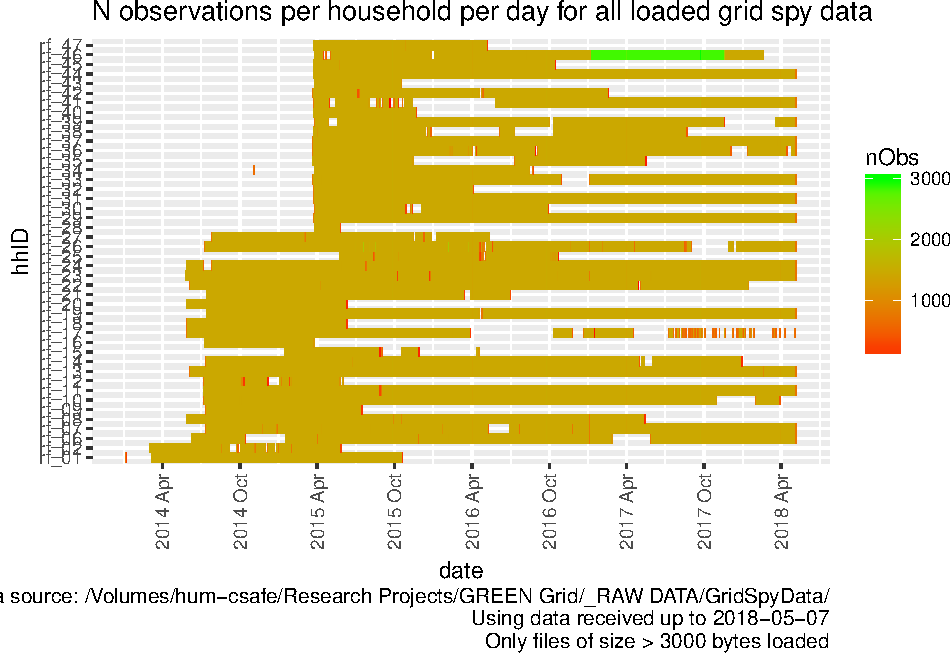
\includegraphics{processNZGGElecCons1minData_files/figure-latex/loadedFilesObsPlots-1.pdf}

\begin{Shaded}
\begin{Highlighting}[]
\KeywordTok{ggsave}\NormalTok{(}\KeywordTok{paste0}\NormalTok{(outPath, }\StringTok{"gridSpyLoadedFileNobsTilePlot.png"}\NormalTok{))}
\end{Highlighting}
\end{Shaded}

\begin{verbatim}
## Saving 6.5 x 4.5 in image
\end{verbatim}

\begin{Shaded}
\begin{Highlighting}[]
\CommentTok{# point plot ----}
\KeywordTok{ggplot}\NormalTok{(hhStatDT, }\KeywordTok{aes}\NormalTok{( }\DataTypeTok{x =}\NormalTok{ date, }\DataTypeTok{y =}\NormalTok{ nObs, }\DataTypeTok{colour =}\NormalTok{ hhID)) }\OperatorTok{+}
\StringTok{  }\KeywordTok{geom_point}\NormalTok{() }\OperatorTok{+}
\StringTok{  }\KeywordTok{scale_x_date}\NormalTok{(}\DataTypeTok{date_labels =} \StringTok{"%Y %b"}\NormalTok{, }\DataTypeTok{date_breaks =} \StringTok{"6 months"}\NormalTok{) }\OperatorTok{+}
\StringTok{  }\KeywordTok{theme}\NormalTok{(}\DataTypeTok{axis.text.x =} \KeywordTok{element_text}\NormalTok{(}\DataTypeTok{angle =} \DecValTok{90}\NormalTok{, }\DataTypeTok{vjust =} \FloatTok{0.5}\NormalTok{, }\DataTypeTok{hjust =} \FloatTok{0.5}\NormalTok{)) }\OperatorTok{+}\StringTok{ }
\StringTok{  }\KeywordTok{labs}\NormalTok{(}\DataTypeTok{title =} \StringTok{"N observations per household per day for all loaded grid spy data"}\NormalTok{,}
       \DataTypeTok{caption =} \KeywordTok{paste0}\NormalTok{(myCaption,}
                        \StringTok{"}\CharTok{\textbackslash{}n}\StringTok{Only files of size > "}\NormalTok{, dataThreshold, }\StringTok{" bytes loaded"}\NormalTok{)}
       
\NormalTok{  )}
\end{Highlighting}
\end{Shaded}

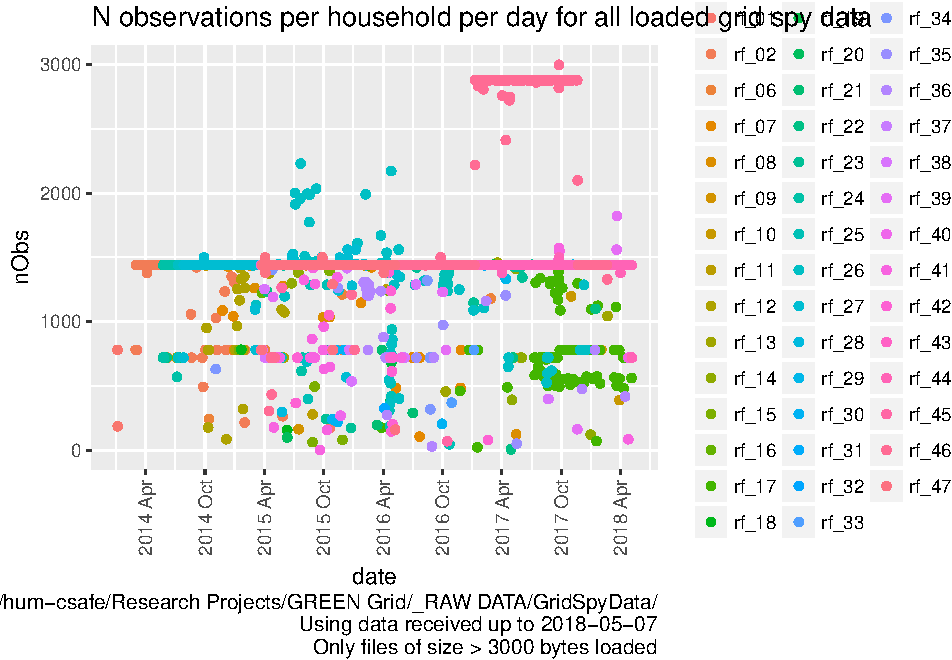
\includegraphics{processNZGGElecCons1minData_files/figure-latex/loadedFilesObsPlots-2.pdf}

\begin{Shaded}
\begin{Highlighting}[]
\KeywordTok{ggsave}\NormalTok{(}\KeywordTok{paste0}\NormalTok{(outPath, }\StringTok{"gridSpyLoadedFileNobsPointPlot.png"}\NormalTok{))}
\end{Highlighting}
\end{Shaded}

\begin{verbatim}
## Saving 6.5 x 4.5 in image
\end{verbatim}

The following table shows the min/max observations per day and min/max
dates for each household. As above, we should not see:

\begin{itemize}
\tightlist
\item
  dates before 2014 or in to the future (indicates date conversion
  errors)
\item
  more than 1440 observations per day (indicates potentially duplicate
  observations)
\end{itemize}

We should also not see NA in any row (indicates date conversion errors).

If we do see any of these then we still have data cleaning work to do!

\begin{Shaded}
\begin{Highlighting}[]
\CommentTok{# Stats table (so we can pick out the dateTime errors)}
\NormalTok{t <-}\StringTok{ }\NormalTok{hhStatDT[, .(}\DataTypeTok{minObs =} \KeywordTok{min}\NormalTok{(nObs),}
             \DataTypeTok{maxObs =} \KeywordTok{max}\NormalTok{(nObs), }\CommentTok{# should not be more than 1440, if so suggests duplicates}
             \DataTypeTok{minDate =} \KeywordTok{min}\NormalTok{(date),}
             \DataTypeTok{maxDate =} \KeywordTok{max}\NormalTok{(date)),}
\NormalTok{         keyby =}\StringTok{ }\NormalTok{.(hhID)]}

\KeywordTok{kable}\NormalTok{(}\DataTypeTok{caption =} \StringTok{"Summary observation stats by hhID"}\NormalTok{, t)}
\end{Highlighting}
\end{Shaded}

\begin{longtable}[]{@{}lrrll@{}}
\caption{Summary observation stats by hhID}\tabularnewline
\toprule
hhID & minObs & maxObs & minDate & maxDate\tabularnewline
\midrule
\endfirsthead
\toprule
hhID & minObs & maxObs & minDate & maxDate\tabularnewline
\midrule
\endhead
rf\_01 & 171 & 1500 & 2014-01-05 & 2015-10-20\tabularnewline
rf\_02 & 215 & 1440 & 2014-03-02 & 2015-05-28\tabularnewline
rf\_06 & 243 & 1500 & 2014-06-08 & 2018-04-29\tabularnewline
rf\_27 & 567 & 1560 & 2014-07-27 & 2016-05-13\tabularnewline
\bottomrule
\end{longtable}

\section{Runtime}\label{runtime}

\begin{Shaded}
\begin{Highlighting}[]
\NormalTok{t <-}\StringTok{ }\KeywordTok{proc.time}\NormalTok{() }\OperatorTok{-}\StringTok{ }\NormalTok{startTime}

\NormalTok{elapsed <-}\StringTok{ }\NormalTok{t[[}\DecValTok{3}\NormalTok{]]}
\end{Highlighting}
\end{Shaded}

Analysis completed in 219.298 seconds ( 3.65 minutes) using
\href{https://cran.r-project.org/package=knitr}{knitr} in
\href{http://www.rstudio.com}{RStudio} with R version 3.4.4 (2018-03-15)
running on x86\_64-apple-darwin15.6.0.

\section{R environment}\label{r-environment}

R packages used:

\begin{itemize}
\tightlist
\item
  base R - for the basics {[}@baseR{]}
\item
  data.table - for fast (big) data handling {[}@data.table{]}
\item
  ggplot2 - for slick graphics {[}@ggplot2{]}
\item
  dplyr - for rename {[}@dplyr{]}
\item
  lubridate - date manipulation {[}@lubridate{]}
\item
  knitr - to create this document {[}@knitr{]}
\item
  greenGridr - for local NZ GREEN Grid utilities
\end{itemize}

\begin{Shaded}
\begin{Highlighting}[]
\KeywordTok{sessionInfo}\NormalTok{()}
\end{Highlighting}
\end{Shaded}

\begin{verbatim}
## R version 3.4.4 (2018-03-15)
## Platform: x86_64-apple-darwin15.6.0 (64-bit)
## Running under: macOS High Sierra 10.13.4
## 
## Matrix products: default
## BLAS: /Library/Frameworks/R.framework/Versions/3.4/Resources/lib/libRblas.0.dylib
## LAPACK: /Library/Frameworks/R.framework/Versions/3.4/Resources/lib/libRlapack.dylib
## 
## locale:
## [1] en_GB.UTF-8/en_GB.UTF-8/en_GB.UTF-8/C/en_GB.UTF-8/en_GB.UTF-8
## 
## attached base packages:
## [1] stats     graphics  grDevices utils     datasets  methods   base     
## 
## other attached packages:
## [1] knitr_1.20          dplyr_0.7.4         readr_1.1.1        
## [4] ggplot2_2.2.1       lubridate_1.7.3     data.table_1.10.4-3
## [7] greenGridr_0.1.0   
## 
## loaded via a namespace (and not attached):
##  [1] Rcpp_0.12.16      bindr_0.1.1       magrittr_1.5     
##  [4] hms_0.4.2         munsell_0.4.3     colorspace_1.3-2 
##  [7] R6_2.2.2          rlang_0.2.0.9001  highr_0.6        
## [10] stringr_1.3.0     plyr_1.8.4        tools_3.4.4      
## [13] grid_3.4.4        gtable_0.2.0      htmltools_0.3.6  
## [16] assertthat_0.2.0  yaml_2.1.18       lazyeval_0.2.1   
## [19] rprojroot_1.3-2   digest_0.6.15     tibble_1.4.2     
## [22] bindrcpp_0.2.2    glue_1.2.0        evaluate_0.10.1  
## [25] rmarkdown_1.9     labeling_0.3      stringi_1.1.7    
## [28] compiler_3.4.4    pillar_1.2.1      scales_0.5.0.9000
## [31] backports_1.1.2   pkgconfig_2.0.1
\end{verbatim}


\end{document}
